\section{Durchführung}
\label{sec:Durchführung}

Es wird eine Schaltung entsprechend Abbildung \ref{fig:Schaltung1} wird aufgebaut.
Es wird jedoch der Noise Generator vorerst ausgelassen. Zudem wurde auch der Pre-Amplifier
nicht mit eingebunden, da dieser offensichtlich nicht einwandfrei funktioniert.
\begin{figure}[H]
  \centering
  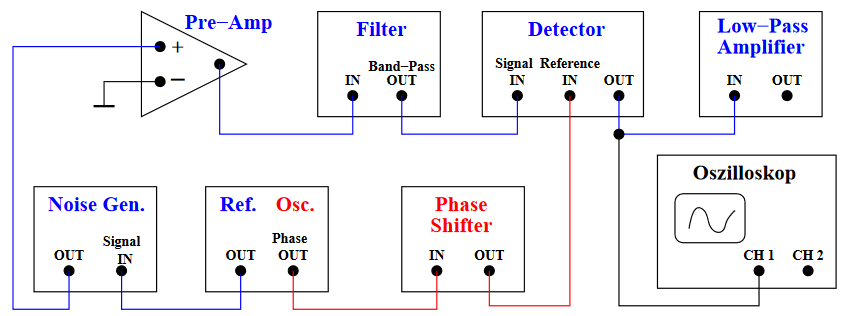
\includegraphics[width=14cm]{Schaltung1.PNG}
  \caption{Schematischer Aufbau eines Lock-In-Verstärkers. \cite{sample}}
  \label{fig:Schaltung1}
\end{figure}

Zu Beginn wird überprüft welche der beiden Ausgänge (Ref./Osc.) eine konstante bzw.
variable Spannung liefert. Da letztere nur vom Ref. Ausgang geliefert wird, wird
dieser als Eingangssignal genutzt. Entsprechend dient die Spannung des Osc. Ausgangs
dann als Referenzsignal.
Nun werden mithilfe des Oszilloskops Bilder der am Detektor abgegriffenen Spannung
bei unterschiedlichen Phasendifferenzen von Signal- und Referenzspannung gemacht.
Anschließend wird der Tiefpass in die Schaltung integriert. Nun wird mit dem Oszilloskop
auch an diesem die Spannung abgegriffen. Die gemessene Ausgangsspannung wird in
Abhängigkeit der Phasendifferenz bei 30 unterschiedlichen Konfigurationen gemessen und notiert.

Anschließend wird mithilfe des Noise Generators ein zusätzliches Störsignal auf die
Signalspannung gegeben. Dieses hat in etwa die gleiche Größenordnung wie die
Signalspannung selbst. Es wird dann eine analoge Messung durchgeführt.

Zuletzt wird eine Schaltung entsprechend Abbildung \ref{fig:Schaltung2} aufgebaut.
\begin{figure}[H]
  \centering
  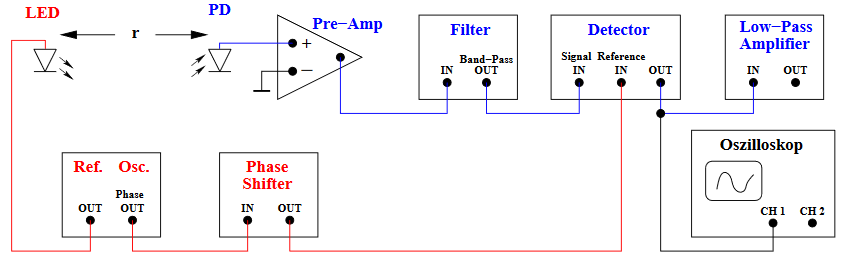
\includegraphics[width=14cm]{Schaltung2.PNG}
  \caption{Aufbau einer Photodetektorschaltung. \cite{sample}}
  \label{fig:Schaltung2}
\end{figure}
Hier dient die an der Photodiode gemessene Spannung als verrauschte Signalspannung.
Die LED selbst wird durch die Spannung am Ref. Ausgang betrieben und blinkt daher
mit der dort angelegten Frequenz.
Es wird die Ausgangsspannung am Detektor in Abhängigkeit des Abstandes von LED zu Photodiode
gemessen. Dazu wird sie an diesem mit dem Oszilloskop abgegriffen und unter Variation des
Abstands abgelesen.
